\iflanguage{english}
{\chapter{Ergebnisse}}
{\chapter{Results}}

\label{sec:results}

In this section, I present the experimental results of my HRHumanTex framework, including both quantitative evaluations and qualitative comparisons. I evaluate the effectiveness of different super-resolution models on UV texture dataset augmentation and analyze the impact of these enhanced inpainting models on the final rendered 3D appearance. I would like to emphasize that in all my visual comparisons of various inpainting evaluation and HRHumanTex variants evaluations, a consistent pseudo-ground-truth, such as PseudoTextureGT and PseudoRenderedGT. This pseudo GT is derived from the original SMPLitex pipeline followed by a super-resolution step using SRFormer, chosen based on my earlier quantitative and qualitative evaluation of different \ac{SOTA} \ac{SR} models. As such, it serves as a refined baseline grounded in SMPLitex.

\begin{table}[h]
\centering
\caption{Rendering-based evaluation of SR models against pseudo-GT. I report average SSIM, LPIPS, their differences from the pseudo-GT, and inverse LPIPS. Dataset from DeepFashion~\cite{liuLQWTcvpr16DeepFashion}.}
\label{tab:render_inv_comparison}
\begin{tabular}{lccccc}
\toprule
\textbf{Model} & \textbf{SSIM}↑ & \textbf{LPIPS}↓ & $\Delta$SSIM & $\Delta$LPIPS & \textbf{Inv-LPIPS}↑ \\
\midrule
HRHumanTex-BSRGAN        & 0.7558 & 0.2830 & +0.00013 & -0.00021 & 0.7170 \\
\maxscore{HRHumanTex-DiffBIR}       & \maxscore{0.7569} & \minscore{0.2832} & \maxscore{+0.00118} & \maxscore{+0.00006} & \minscore{0.7168} \\
PseudoGT                 & 0.7557 & 0.2832 & ---       & ---        & 0.7168 \\
HRHumanTex-RCAN          & 0.7558 & \maxscore{0.2827} & +0.00009 & \minscore{-0.00045} & \maxscore{0.7173} \\
HRHumanTex-RealESRGAN    & 0.7568 & 0.2833 & +0.00108 & +0.00014 & 0.7167 \\
HRHumanTex-StableSR      & 0.7559 & 0.2828 & +0.00018 & -0.00041 & 0.7172 \\
HRHumanTex-SwinIR        & 0.7562 & 0.2829 & +0.00048 & -0.00025 & 0.7171 \\
\bottomrule
\end{tabular}
\end{table}


\begin{table}[h]
\centering
\caption{Comparison of inpainting models evaluated on full-texture quality. Metrics are averaged over 50 samples. Dataset from DeepFashion.}
\label{tab:inpaint_eval1}
\begin{tabular}{lcccc}
\toprule
\textbf{Model} & \textbf{PSNR}↑ & \textbf{SSIM}↑ & \textbf{LPIPS}↓ & \textbf{FID}↓ \\
\midrule
inpaintedBSRGAN        & 15.64 & 0.5708 & 0.4319 & 140.36 \\
inpaintedRealESRGAN    & 15.56 & \maxscore{0.5798} & 0.4532 & \maxscore{136.92} \\
inpaintedSwinIR        & \maxscore{15.74} & 0.5739 & 0.4427 & 143.15 \\
inpaintedSRFormer      & \minscore{15.19} & \minscore{0.5539} & \maxscore{0.4402} & 148.55 \\
inpaintedStableSR      & 15.57 & 0.5618 & 0.4454 & 142.40 \\
inpaintedDiffBIR       & 15.77 & 0.5716 & \minscore{0.4674} & \minscore{147.37} \\
inpaintedRCAN          & 15.62 & 0.5631 & 0.4365 & 139.38 \\
\bottomrule
\end{tabular}
\end{table}

\begin{table}[h]
\centering
\caption{Comparison of inpainting models on $1024^2$ resolution textures. Metrics are computed over rendered views against PGT images. Dataset from SHHQ ~\cite{fu2022styleganhuman}}
\label{tab:inpaint_eval_shhq}
\begin{tabular}{lcccc}
\toprule
\textbf{Model} & \textbf{PSNR}↑ & \textbf{SSIM}↑ & \textbf{LPIPS}↓ & \textbf{FID}↓ \\
\midrule
inpaintedBSRGAN      & 16.48 & 0.5781 & \maxscore{0.4348} & 149.66 \\
inpaintedRealESRGAN  & 16.41 & \maxscore{0.5838} & \minscore{0.4652} & 155.21 \\
\maxscore{inpaintedSwinIR} & \maxscore{16.51} & 0.5744 & 0.4364 & \maxscore{140.74} \\
inpaintedSRFormer    & \minscore{16.29} & \minscore{0.5663} & 0.4446 & \maxscore{147.54} \\
inpaintedDiffBIR     & 16.57 & 0.5783 & \minscore{0.4688} & \minscore{159.51} \\
inpaintedRCAN        & 16.47 & 0.5729 & 0.4390 & 142.15 \\
\bottomrule
\end{tabular}
\end{table}

\begin{table}[h]
\centering
\caption{Comparison of SR models on rendered images (masked evaluation). Metrics averaged over 31 samples from SHHQ~\cite{fu2022styleganhuman}.}
\label{tab:sr_eval_rendered_shhq}
\begin{tabular}{lcccc}
\toprule
\textbf{Model} & \textbf{SSIM}↑ & \textbf{LPIPS}↓ & \textbf{$\Delta$SSIM}↑ & \textbf{$\Delta$LPIPS}↓ \\
\midrule
\maxscore{HRHumanTex-DiffBIR}     & \maxscore{0.8162} & 0.2125 & \maxscore{+0.0016} & -0.0016 \\
HRHumanTex-BSRGAN         & 0.8156 & \maxscore{0.2122} & +0.0010 & \maxscore{-0.0019} \\
HRHumanTex-PseudoGT       & 0.8146 & 0.2141 & ---     & ---     \\
HRHumanTex-RCAN           & 0.8153 & 0.2124 & +0.0007 & -0.0017 \\
HRHumanTex-Real-ESRGAN    & 0.8160 & 0.2136 & +0.0014 & -0.0005 \\
HRHumanTex-StableSR       & 0.8154 & 0.2125 & +0.0008 & -0.0016 \\
\minscore{HRHumanTex-SwinIR}      & \minscore{0.8152} & 0.2126 & +0.0006 & -0.0015 \\
\bottomrule
\end{tabular}
\end{table}



\begin{figure}[ht]
	\centering
	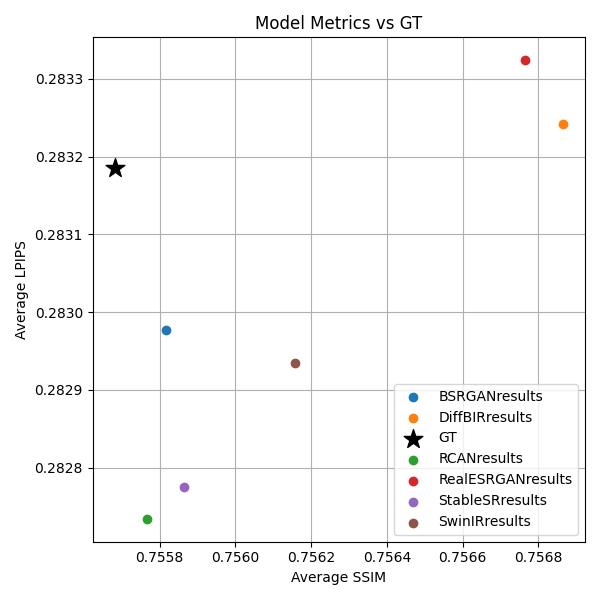
\includegraphics[width=0.6\textwidth]{fig/comparison_scatter_with_gt_df.png}
	\caption{Rendering quantitative analysis results based on different inpainting models, dataset from DeepFashion.}
	\label{fig:inpainteval2}
\end{figure}

\begin{figure}[ht]
	\centering
	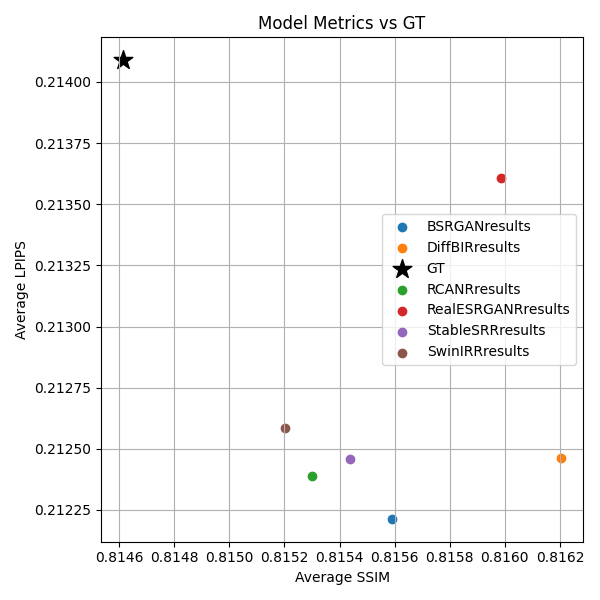
\includegraphics[width=0.6\textwidth]{fig/comparison_scatter_with_gt_shhq.png}
	\caption{Rendering quantitative analysis results based on different inpainting models, dataset from SHHQ.}
	\label{fig:shhqeval2}
\end{figure}

\begin{figure}[ht]
	\centering
    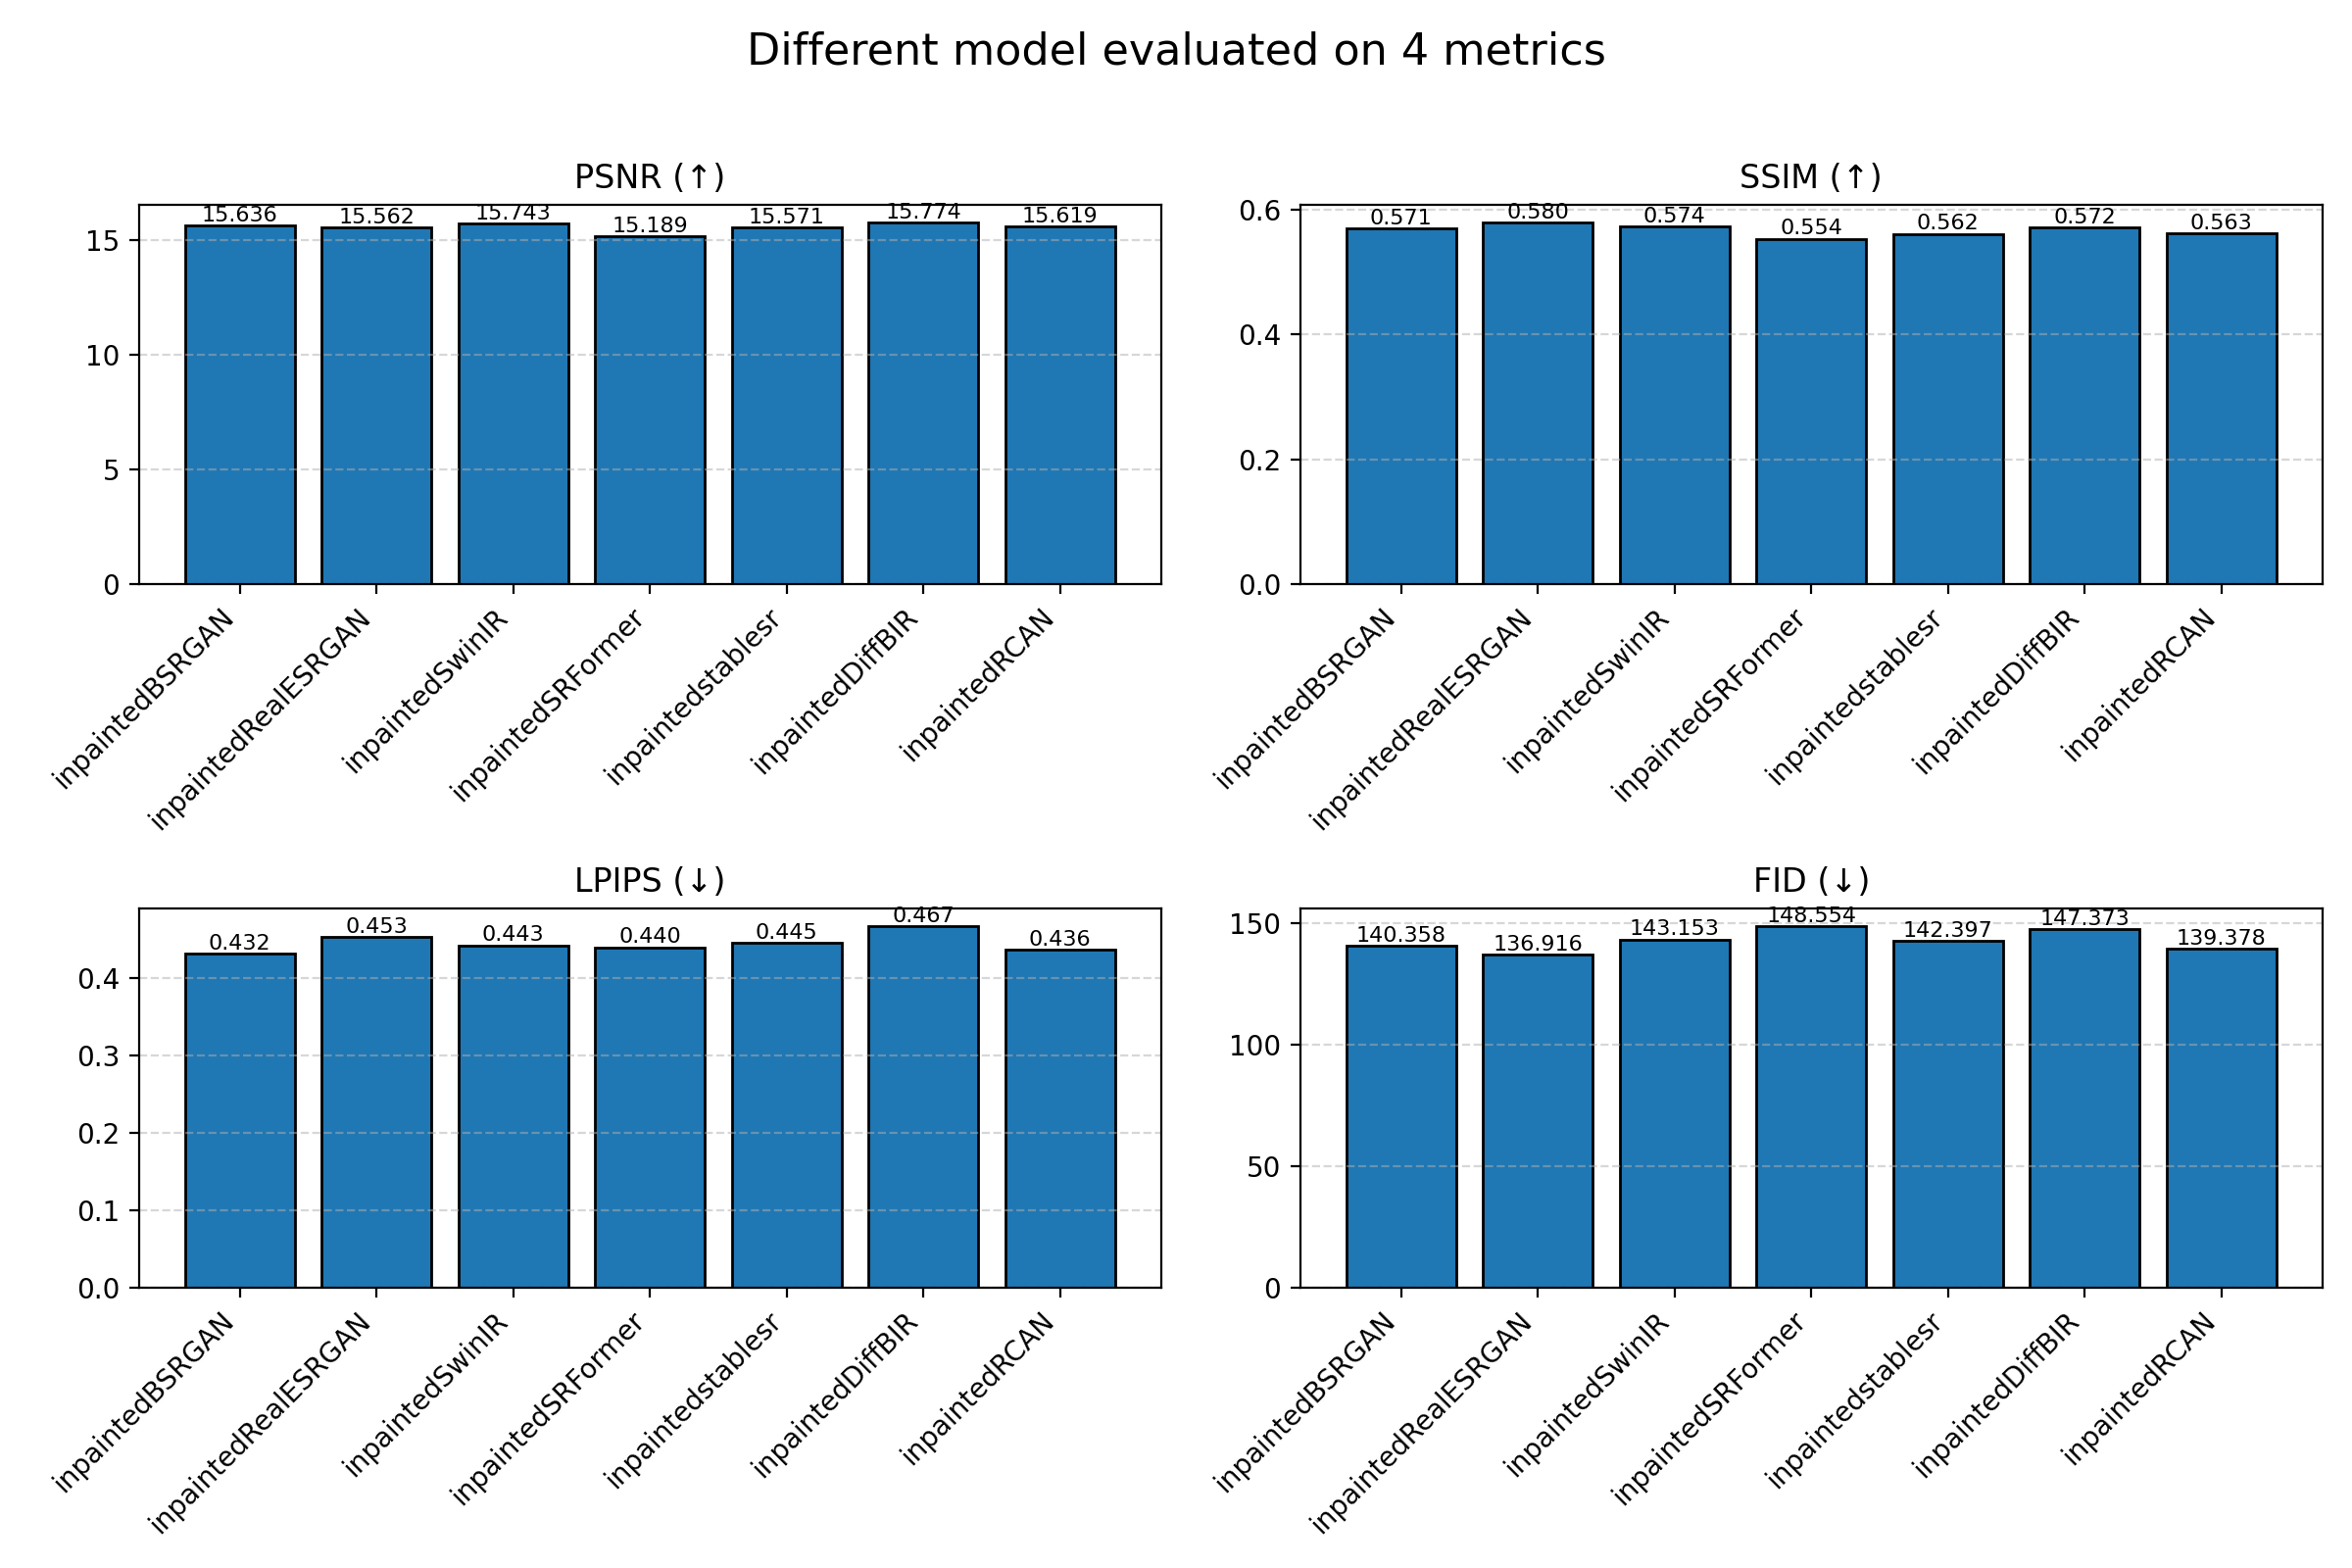
\includegraphics[width=0.9\textwidth]{fig/comparison_4metrics.png}
	\caption{Direct quantitative analysis on different inpainting models in UV space, dataset from DeepFashion.}
	\label{fig:inpainteval2}
\end{figure}

\begin{figure}[ht]
	\centering
    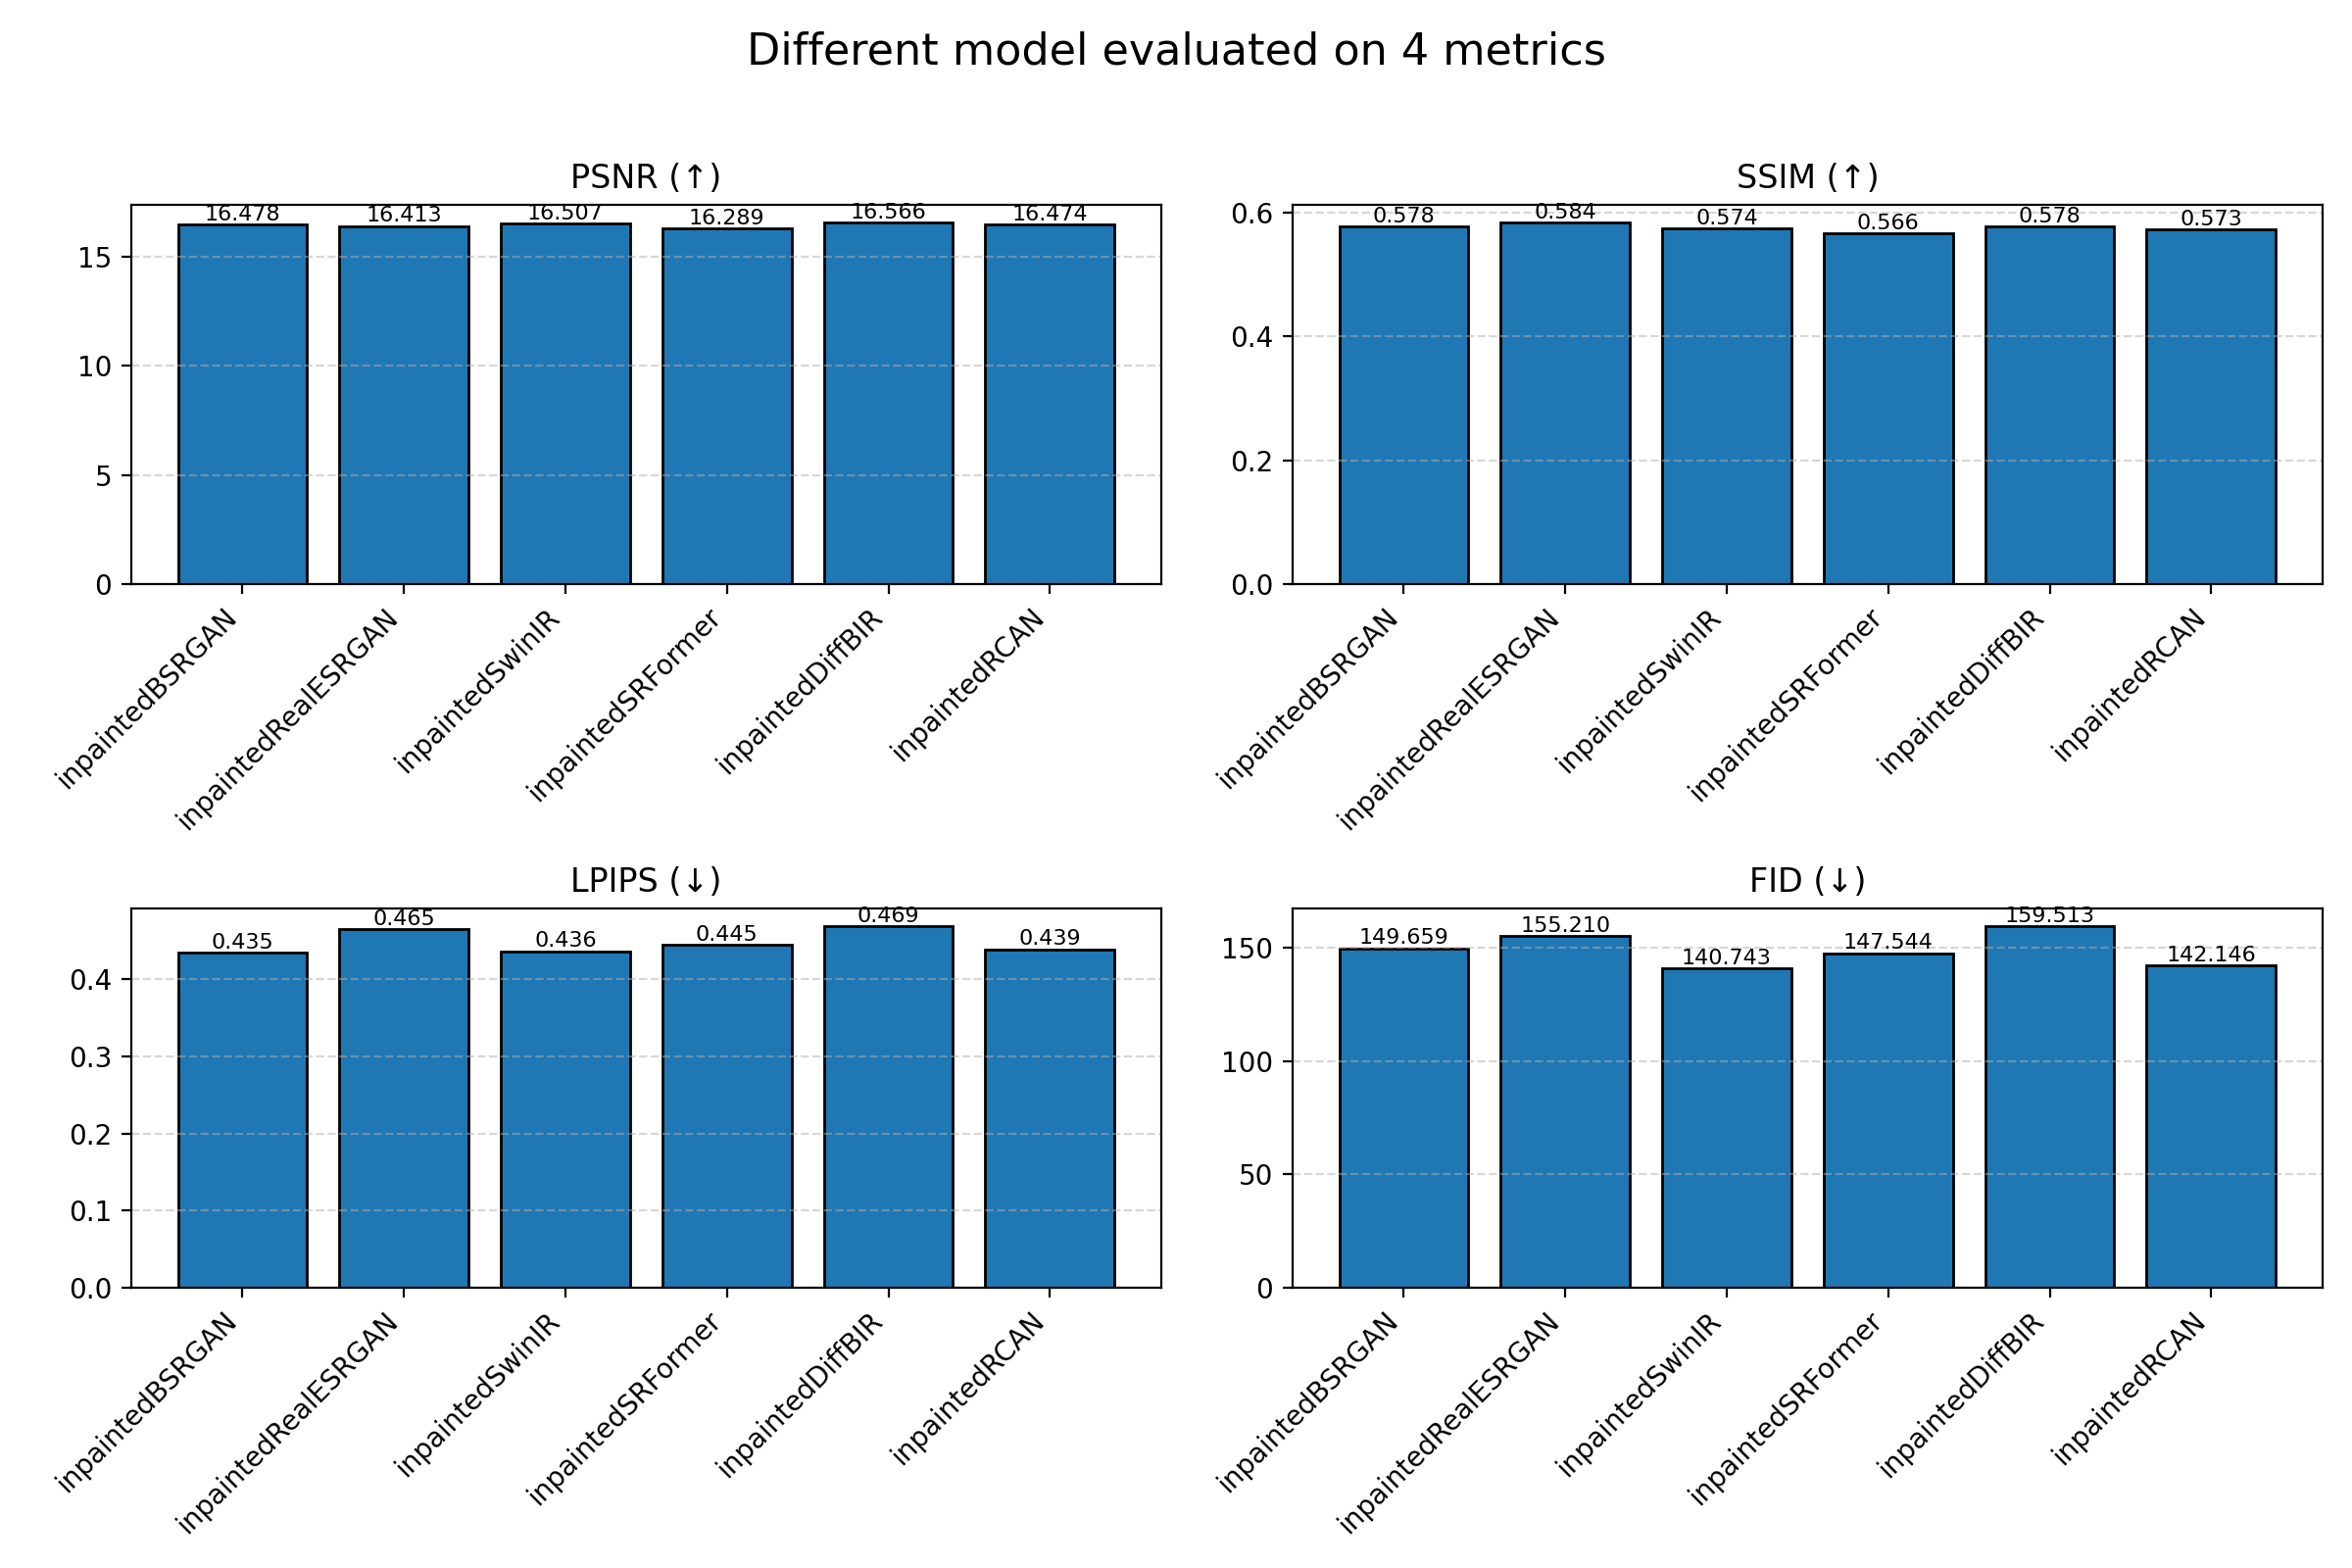
\includegraphics[width=0.9\textwidth]{fig/comparison_4metrics_shhq.png}
	\caption{Direct quantitative analysis on different inpainting models in UV space, dataset from SHHQ.}
	\label{fig:shhqeval}
\end{figure}

\begin{figure}[ht]
	\centering
	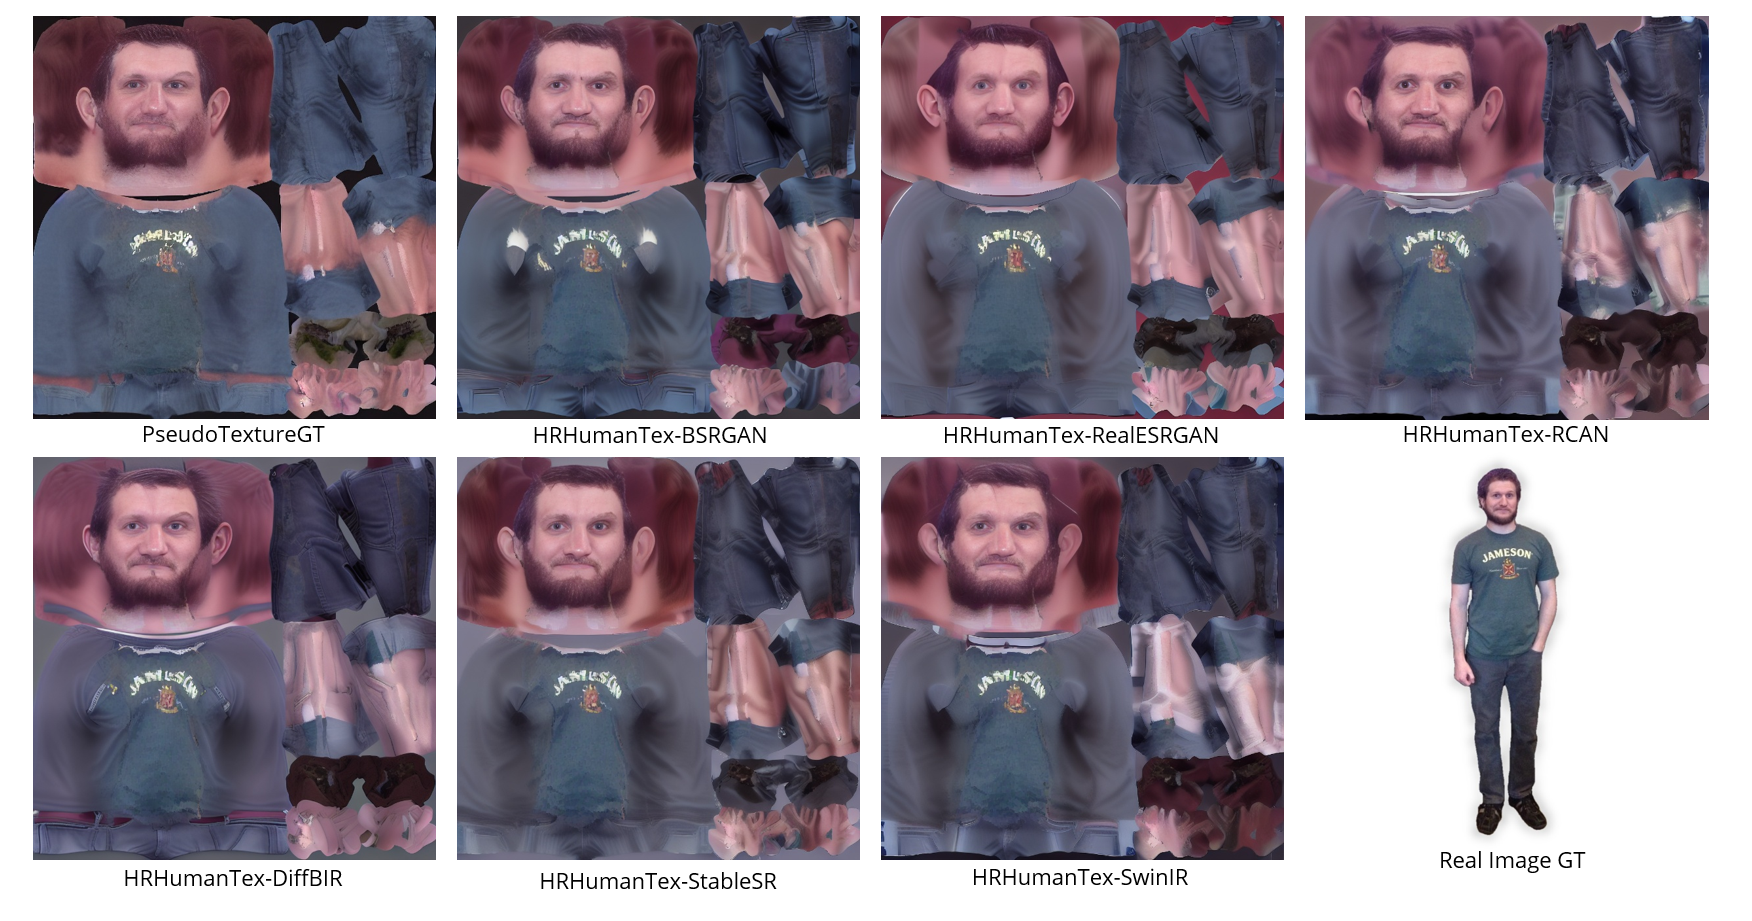
\includegraphics[width=1\textwidth]{fig/shhq2.png}
    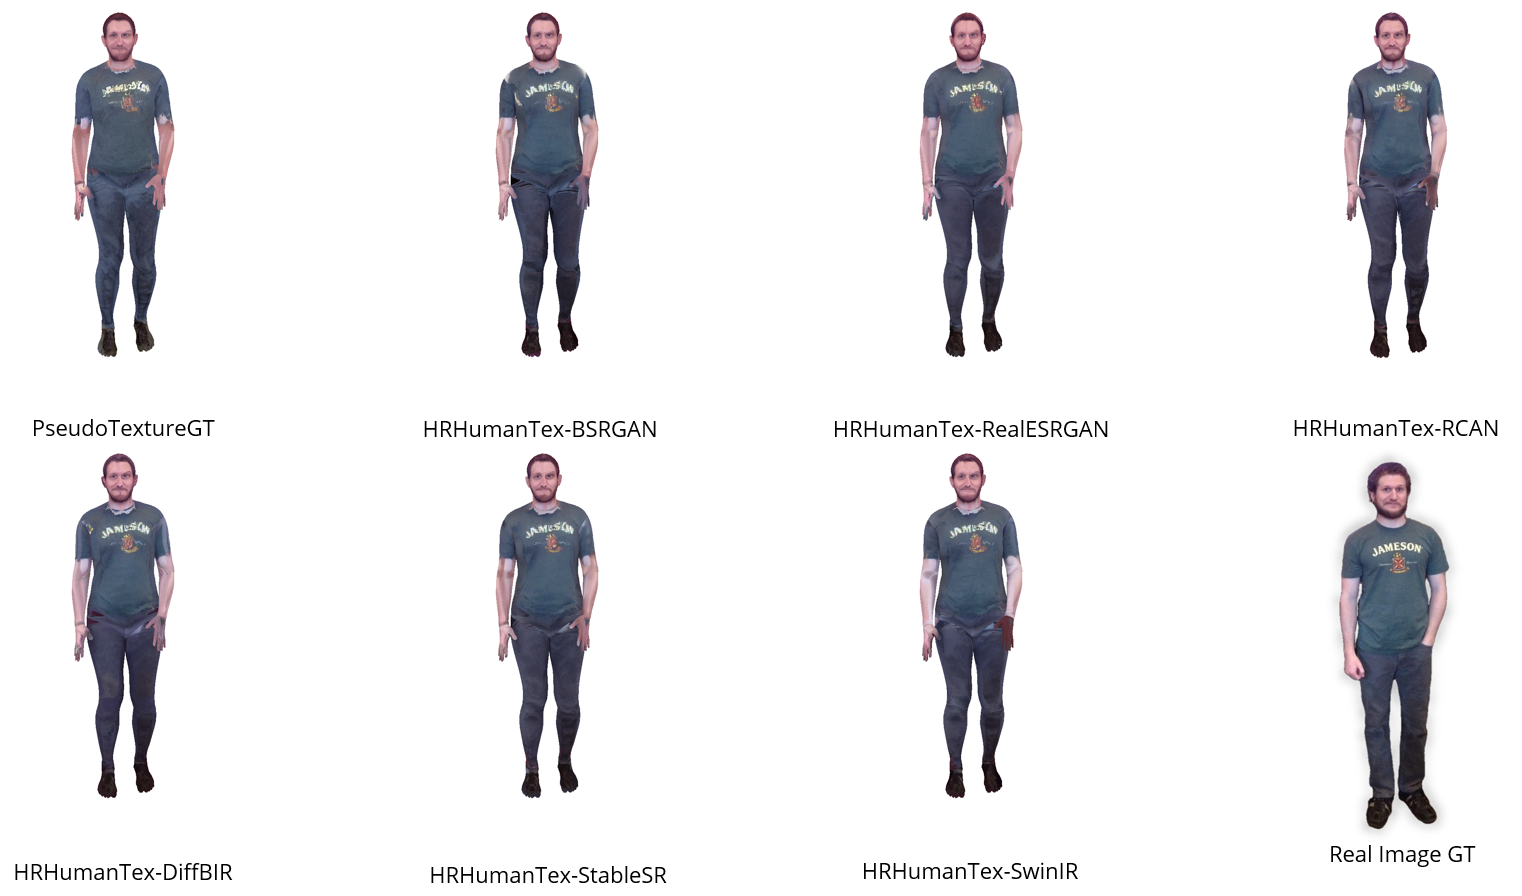
\includegraphics[width=1\textwidth]{fig/shhq6.png}
	\caption{ More qualitative visual comparison of different inpainting models in UV space and rendered images, data sampled from dataset SHHQ-1.0 from~\cite{fu2022styleganhuman}.}
	\label{fig:shhqvisual1}
\end{figure}

\begin{figure}[ht]
	\centering
    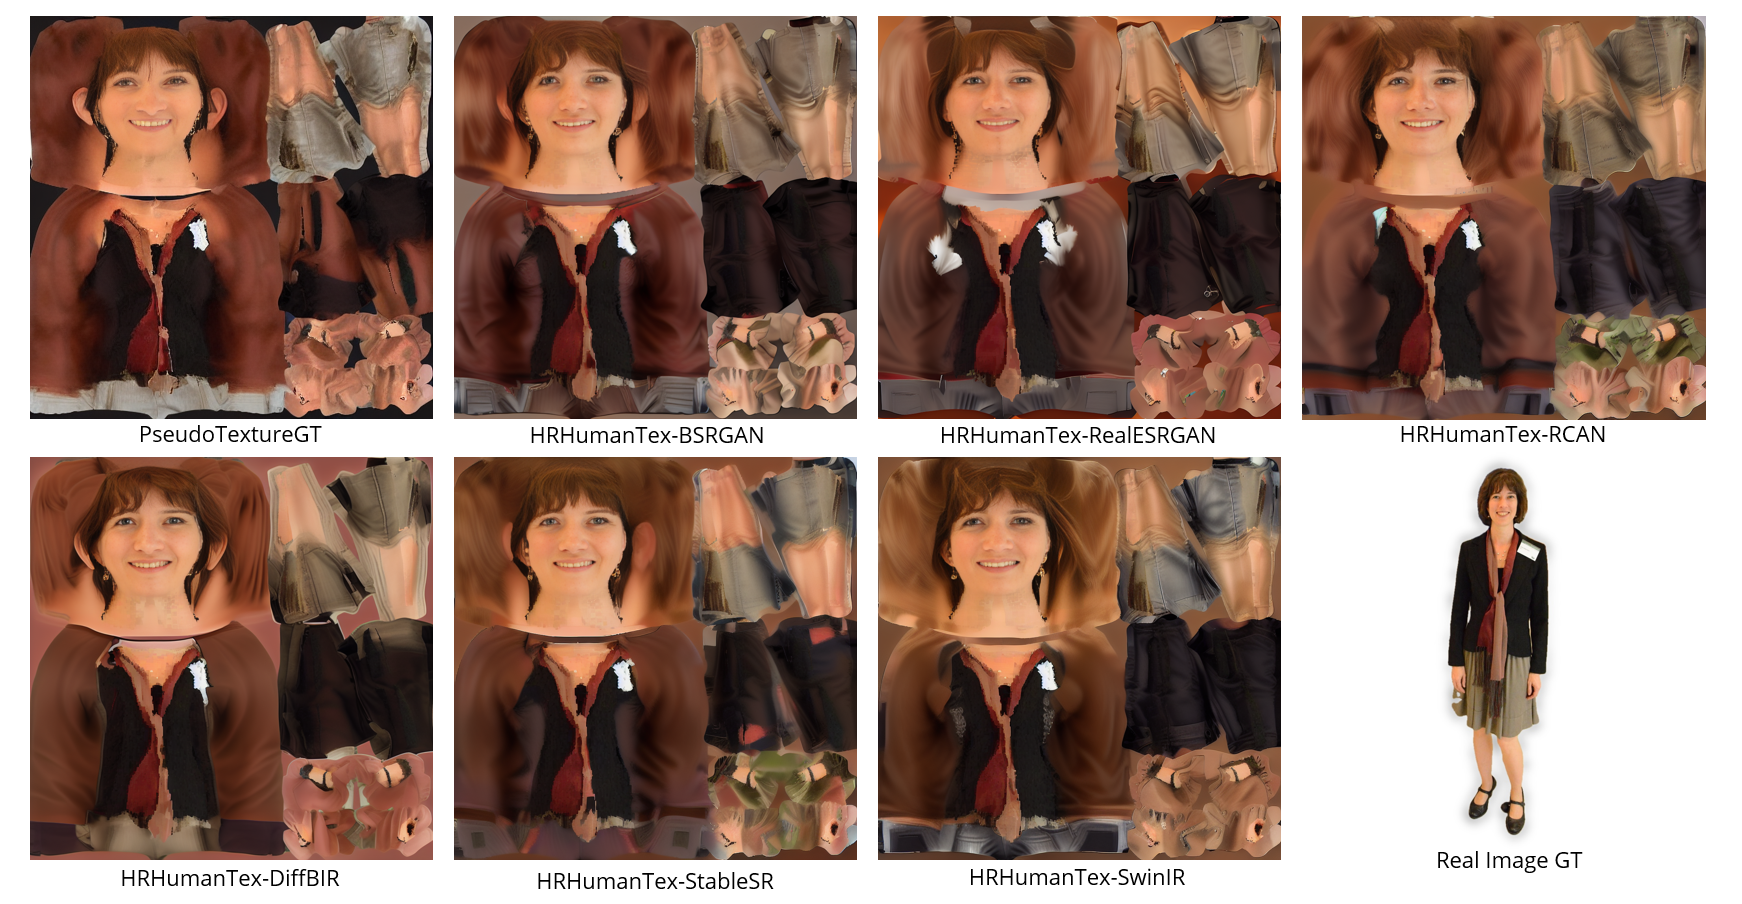
\includegraphics[width=1\textwidth]{fig/shhq3.png}
    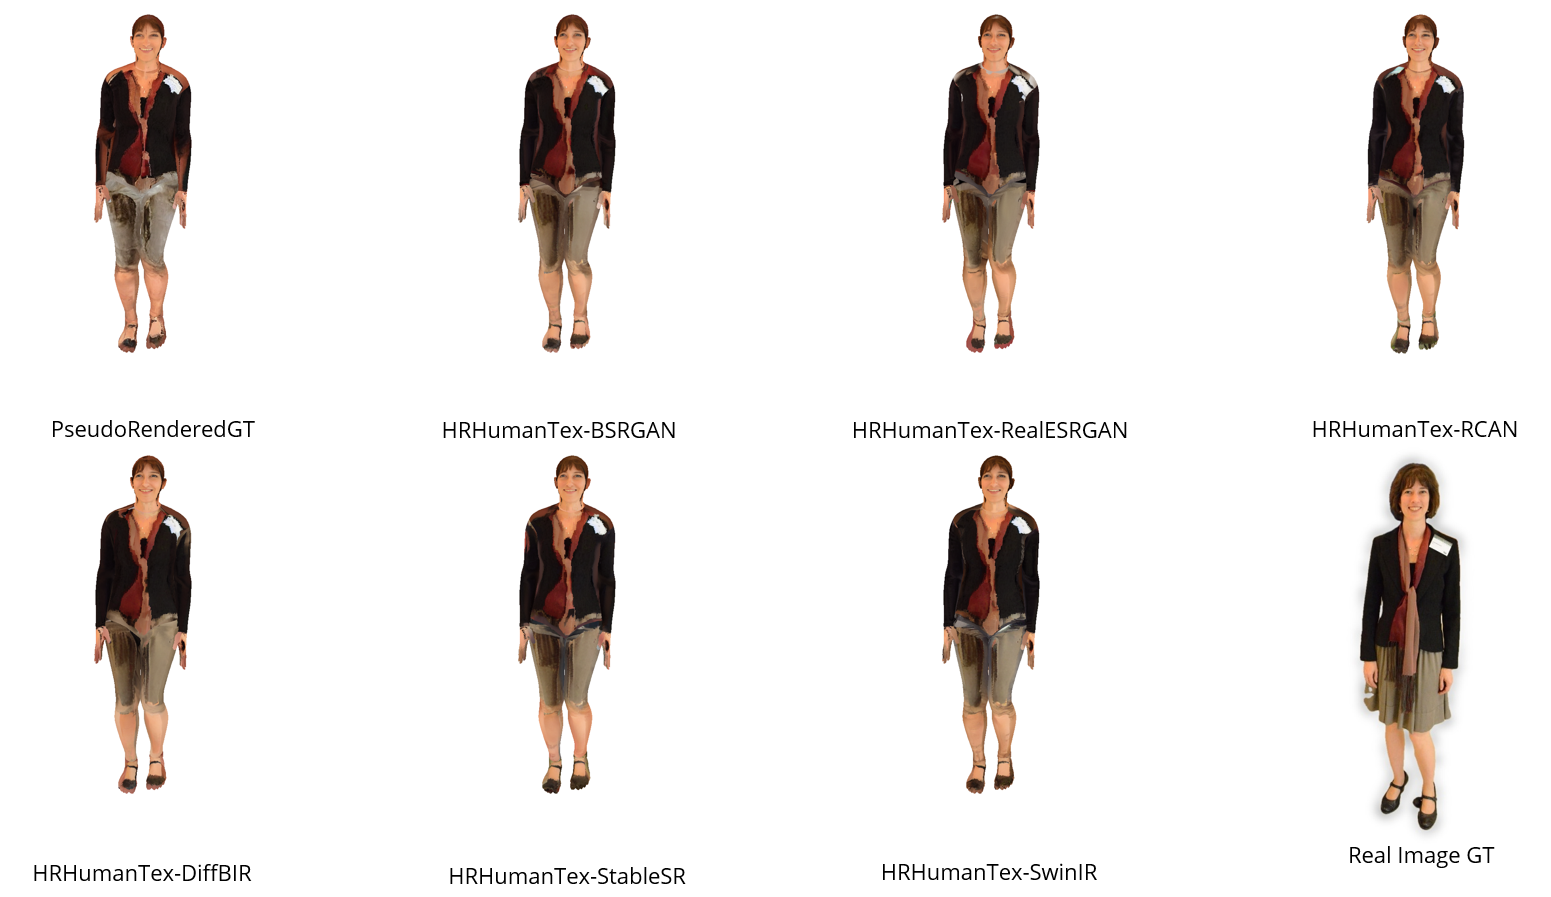
\includegraphics[width=1\textwidth]{fig/shhq8.png}
	\caption{ More qualitative visual comparison of different inpainting models in UV space and rendered images, data sampled from dataset SHHQ-1.0 from~\cite{fu2022styleganhuman}.}
	\label{fig:shhqvisual2}
\end{figure}

\begin{figure}[ht]
	\centering
    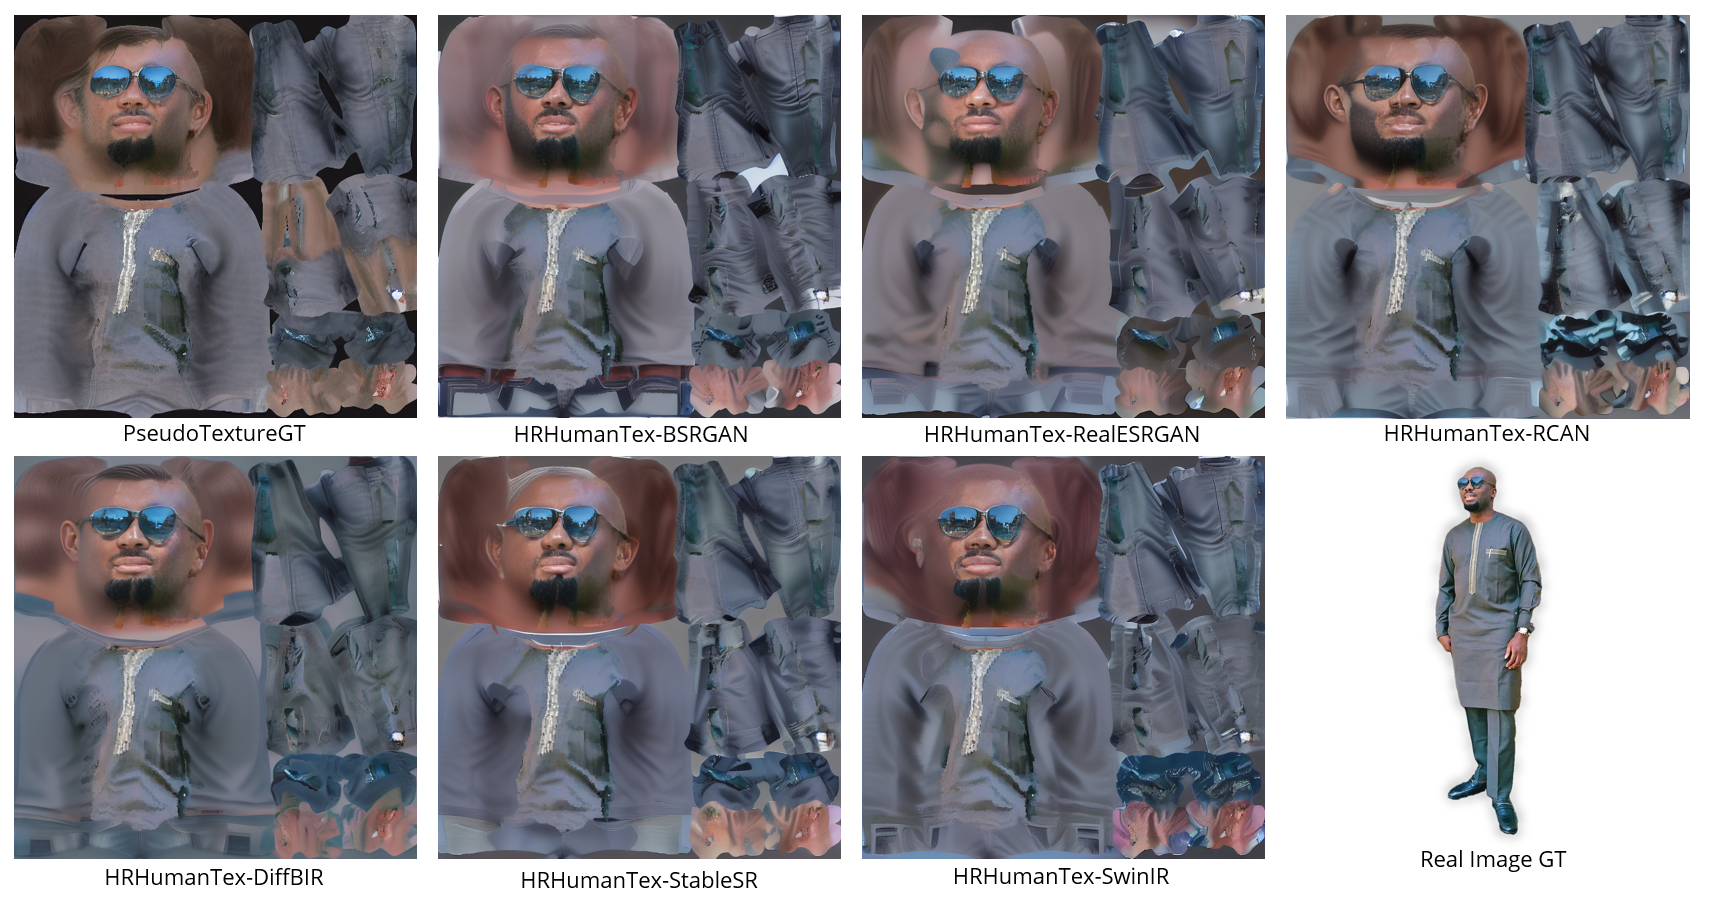
\includegraphics[width=1\textwidth]{fig/shhq4.png}
    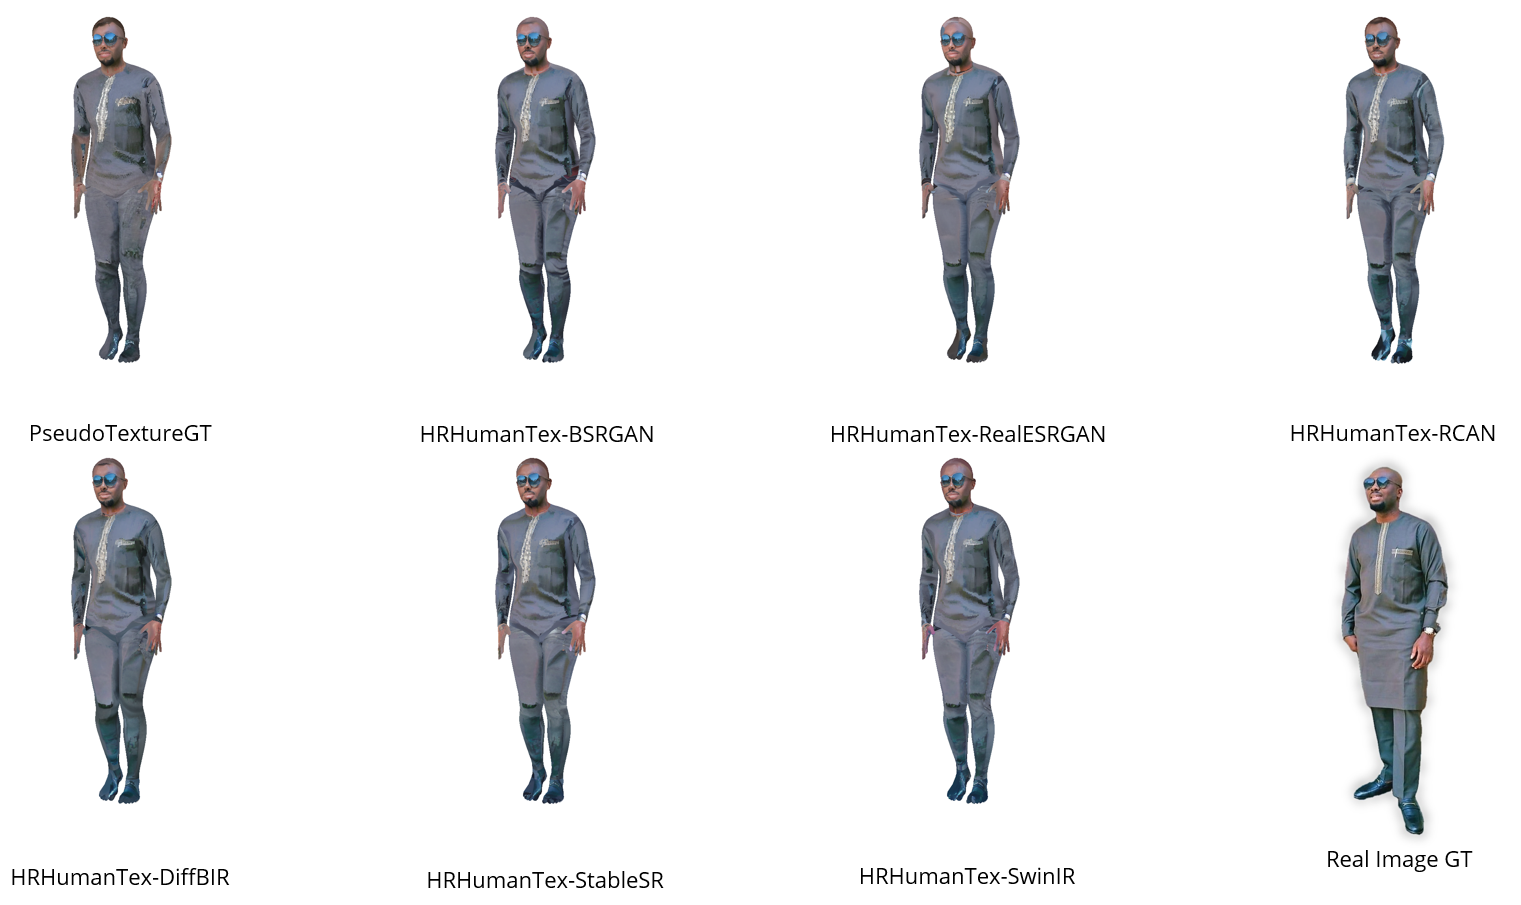
\includegraphics[width=1\textwidth]{fig/shhq9.png}
	\caption{ More qualitative visual comparison of different inpainting models in UV space and rendered images, data sampled from dataset SHHQ-1.0 from~\cite{fu2022styleganhuman}.}
	\label{fig:shhqvisual3}
\end{figure}

\begin{figure}[ht]
	\centering
    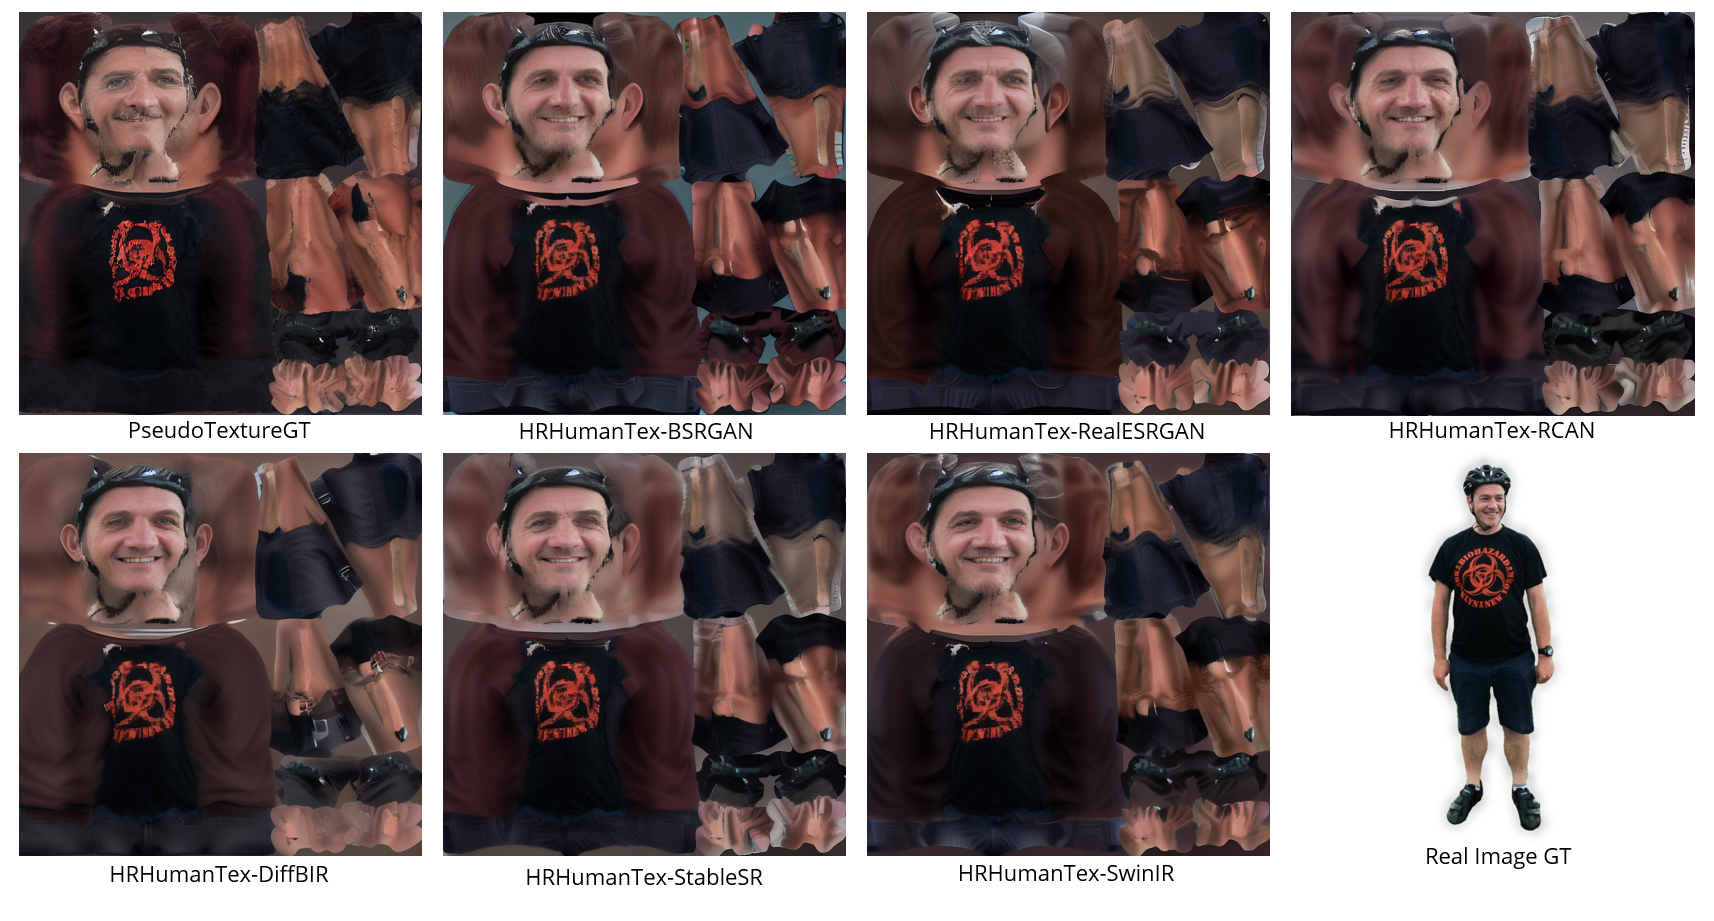
\includegraphics[width=1\textwidth]{fig/shhq5.png}
    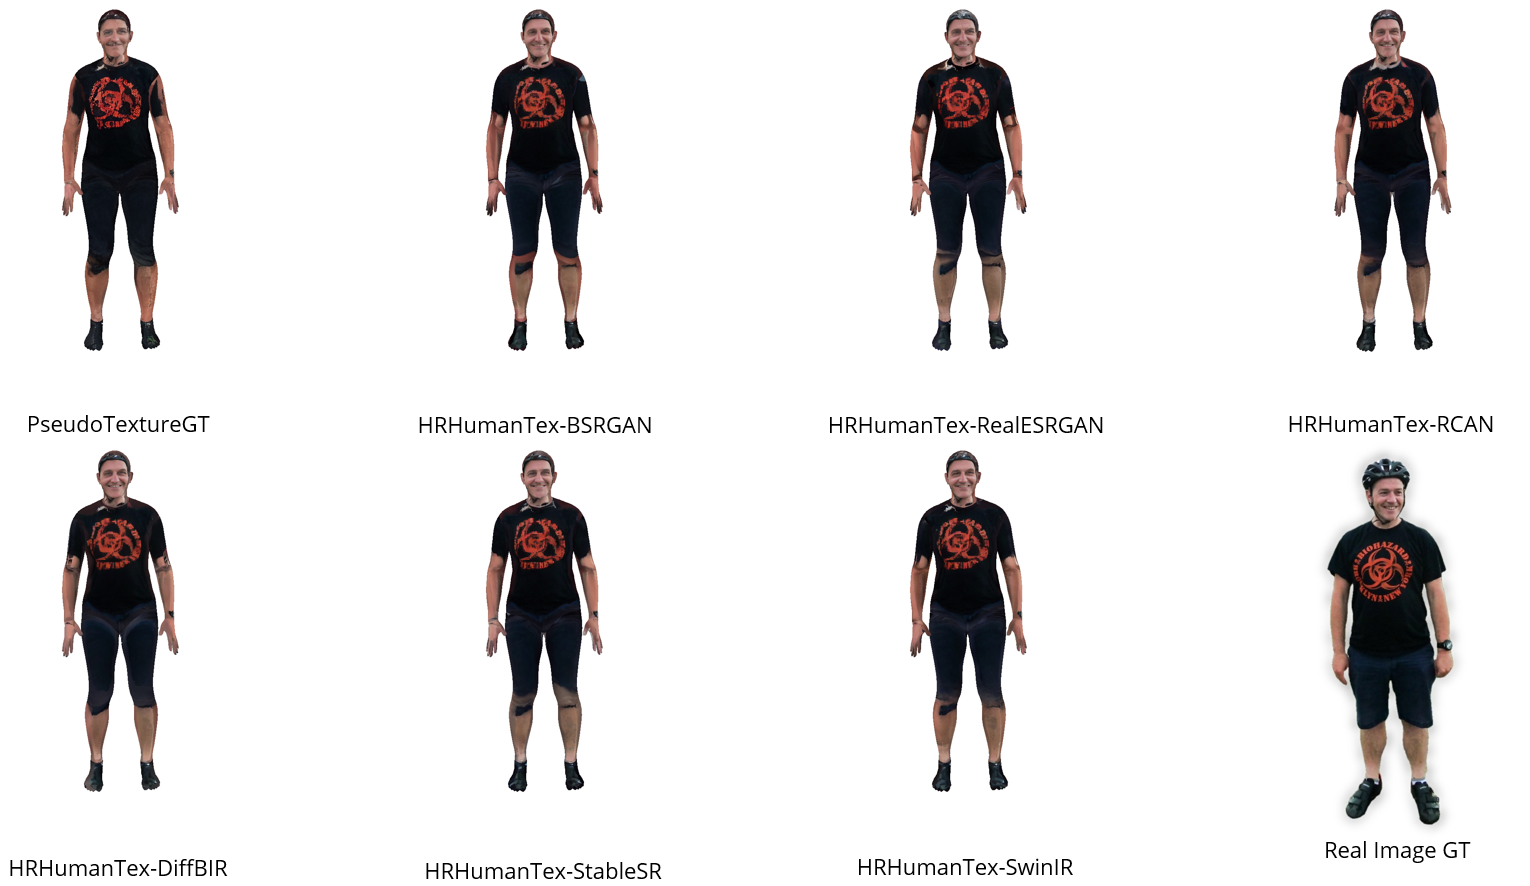
\includegraphics[width=1\textwidth]{fig/shhq10.png}
	\caption{ More qualitative visual comparison of different inpainting models in UV space and rendered images, data sampled from dataset SHHQ-1.0 from~\cite{fu2022styleganhuman}.}
	\label{fig:shhqvisual4}
\end{figure}

\begin{figure}[ht]
	\centering
    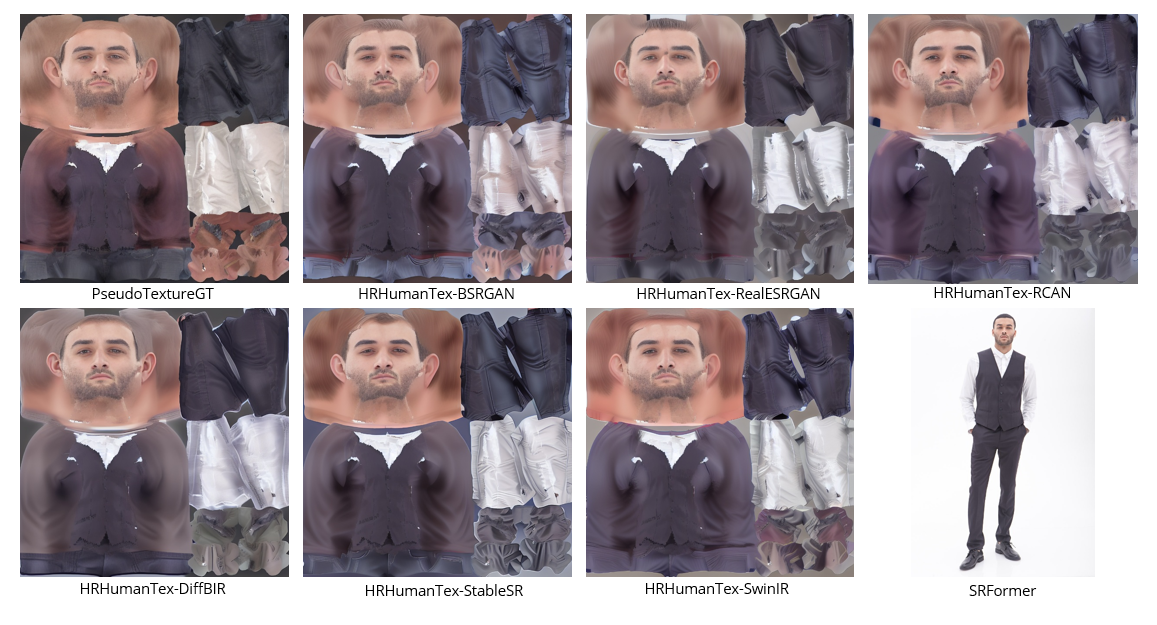
\includegraphics[width=1\textwidth]{fig/df3.png}
    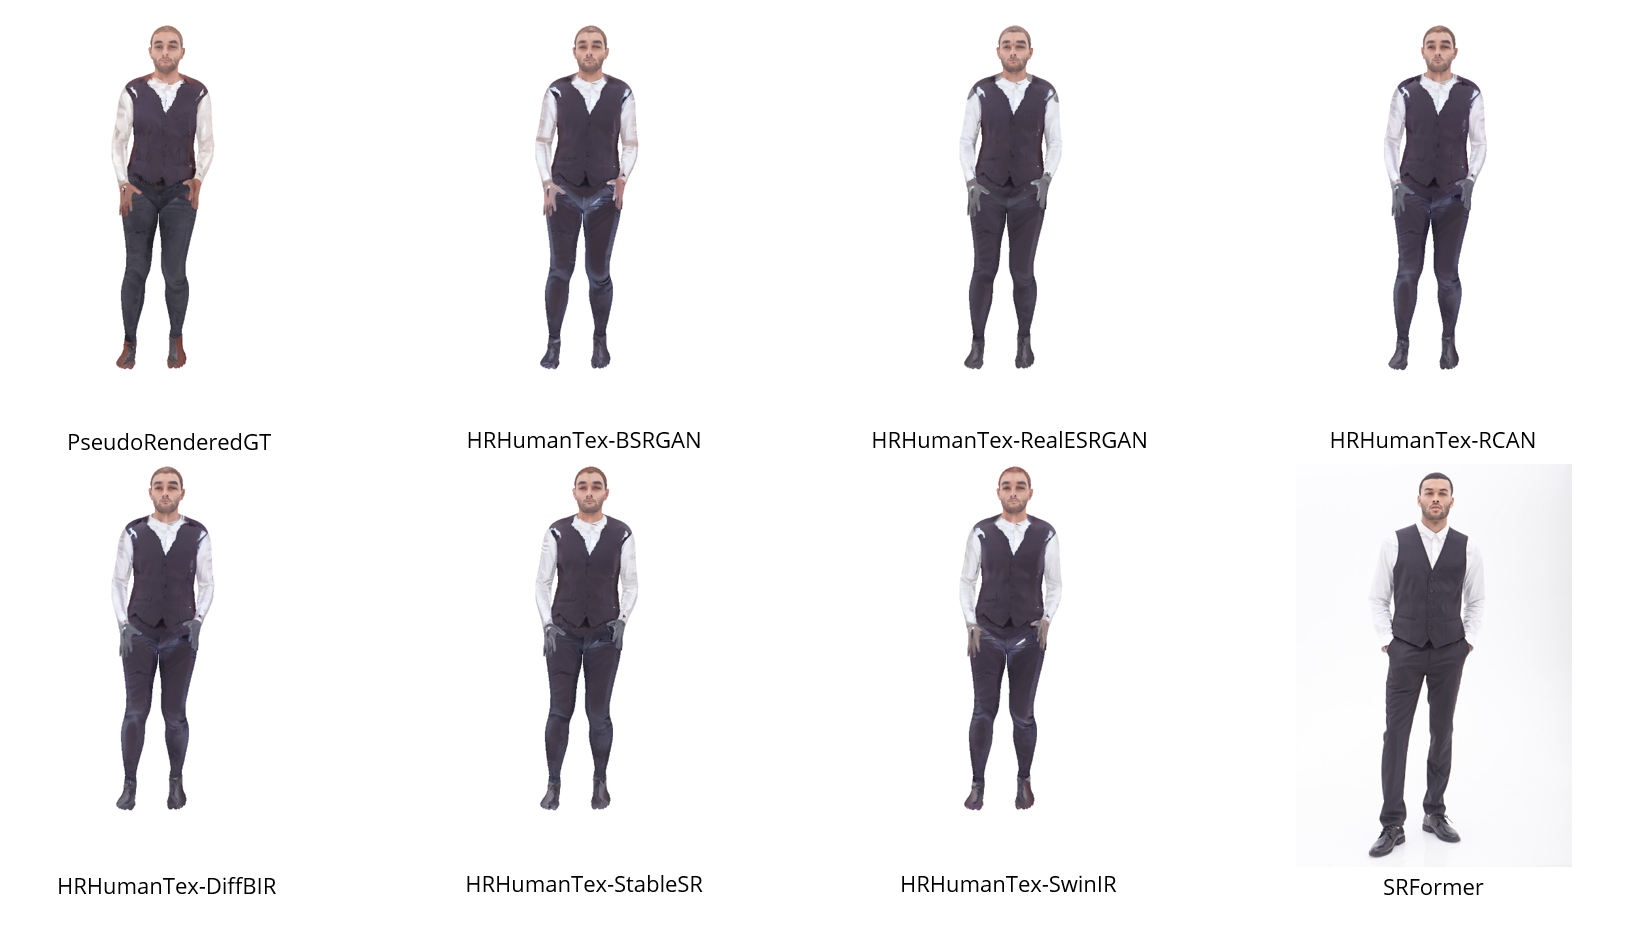
\includegraphics[width=1\textwidth]{fig/df4.png}
	\caption{ More qualitative visual comparison of different inpainting models in UV space and rendered images, data sampled from dataset DeepFashion~\cite{liuLQWTcvpr16DeepFashion}.}
	\label{fig:dfvis1}
\end{figure}

\begin{figure}[ht]
	\centering
    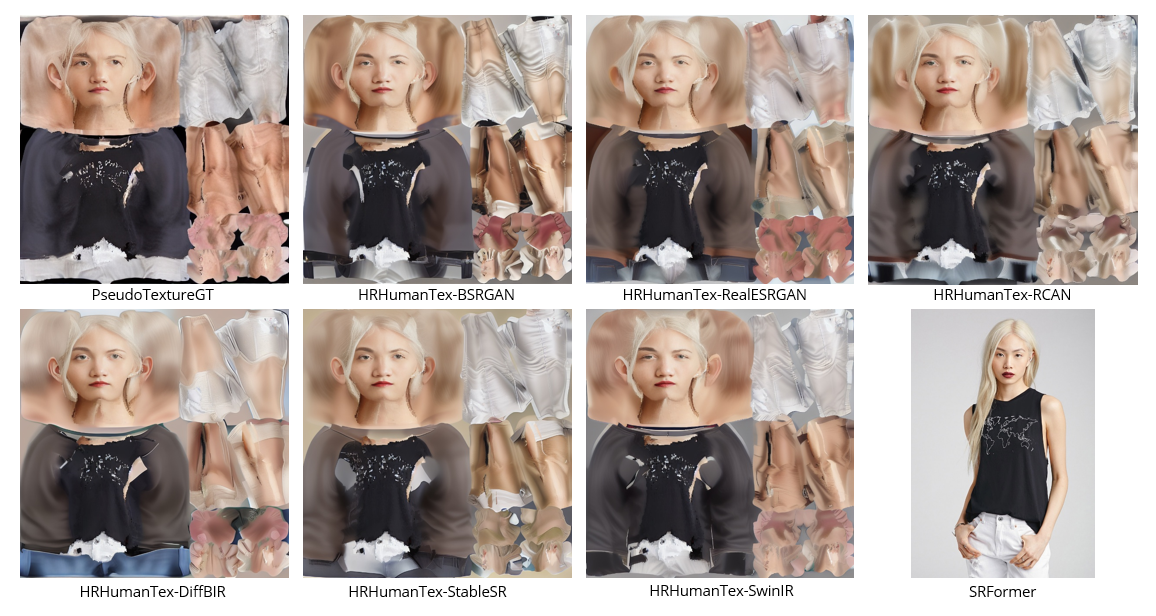
\includegraphics[width=1\textwidth]{fig/df5.png}
    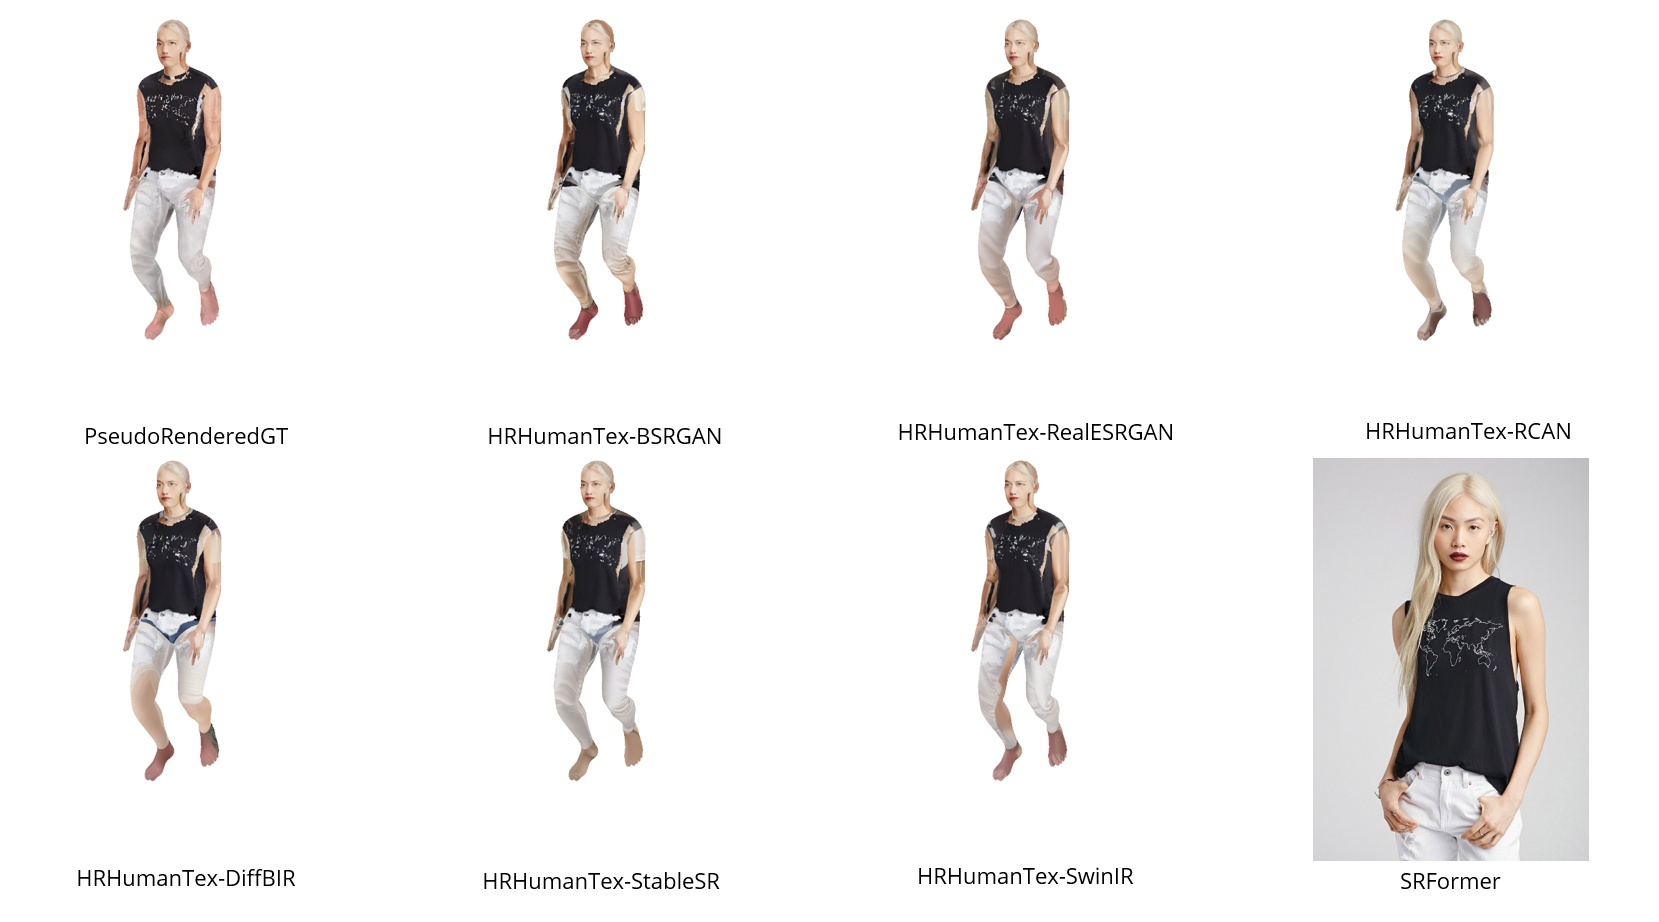
\includegraphics[width=1\textwidth]{fig/df6.png}
	\caption{ More qualitative visual comparison of different inpainting models in UV space and rendered images, data sampled from dataset DeepFashion~\cite{liuLQWTcvpr16DeepFashion}.}
	\label{fig:dfvis2}
\end{figure}

\begin{figure}[ht]
	\centering
    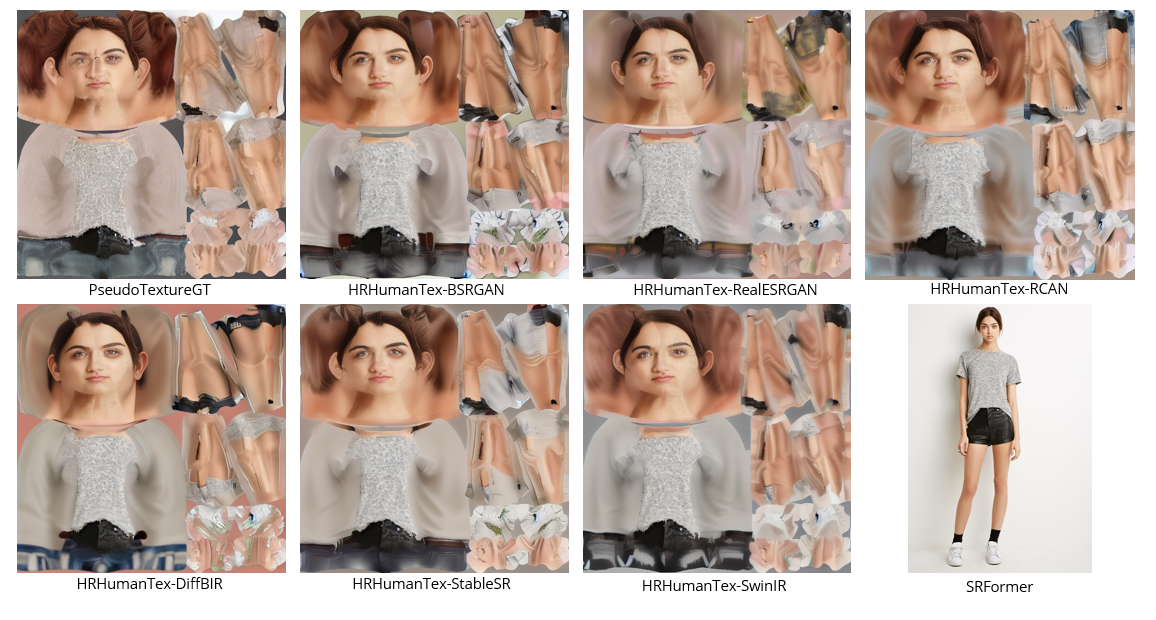
\includegraphics[width=1\textwidth]{fig/df7.png}
    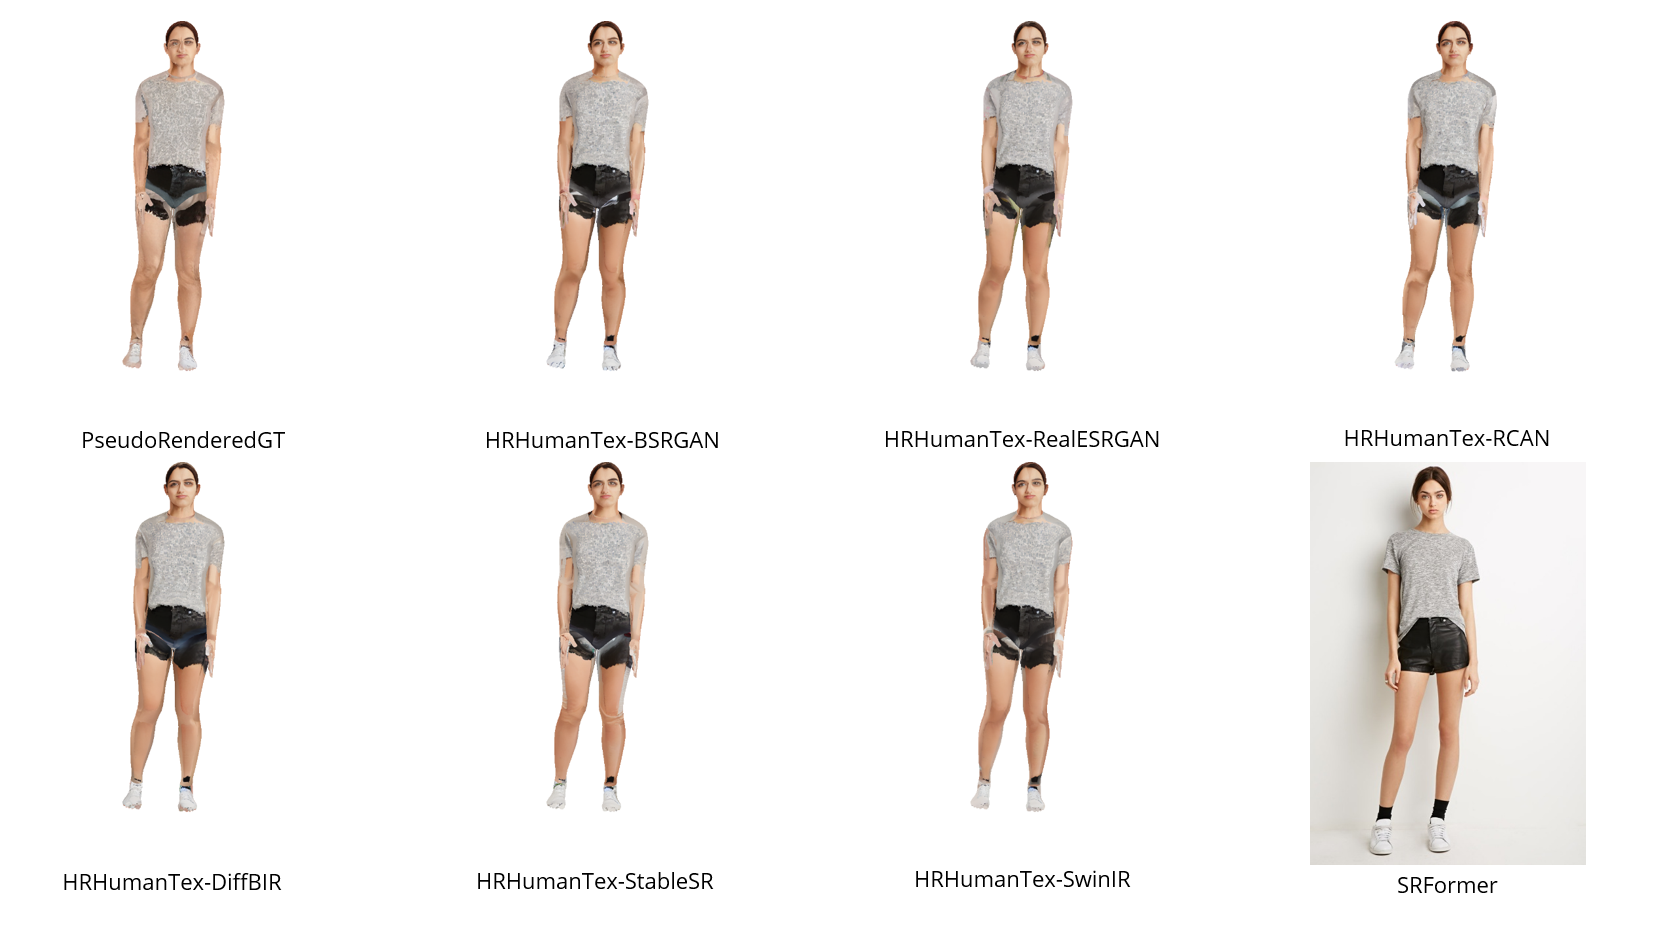
\includegraphics[width=1\textwidth]{fig/df8.png}
	\caption{ More qualitative visual comparison of different inpainting models in UV space and rendered images, data sampled from dataset DeepFashion~\cite{liuLQWTcvpr16DeepFashion}.}
	\label{fig:dfvis3}
\end{figure}

\begin{figure}[ht]
	\centering
    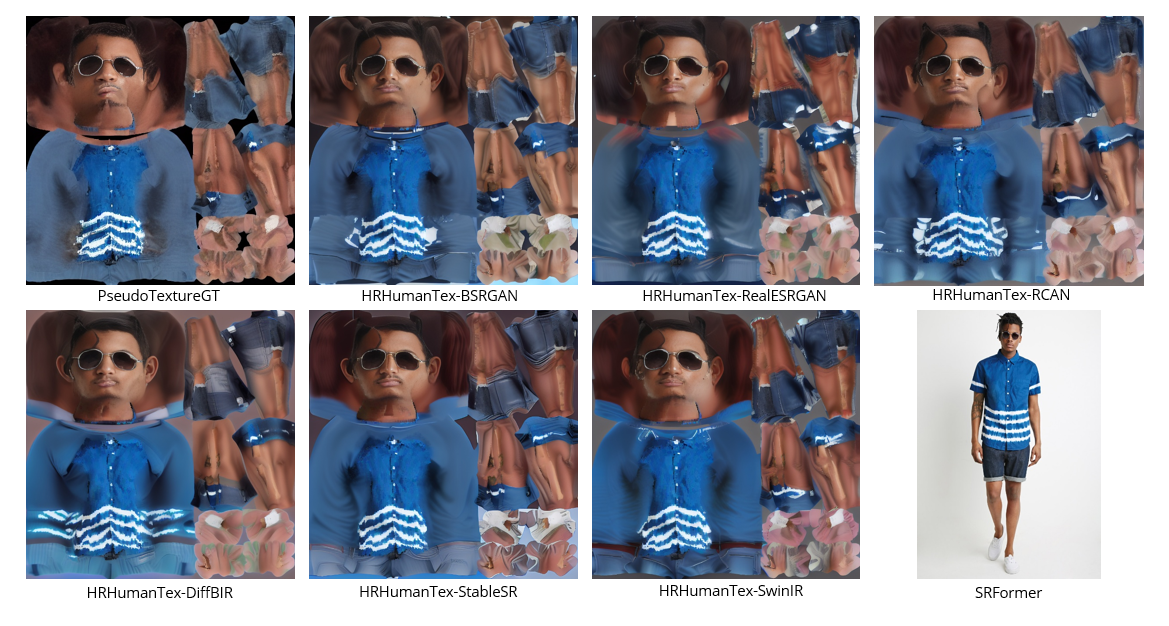
\includegraphics[width=1\textwidth]{fig/df9.png}
    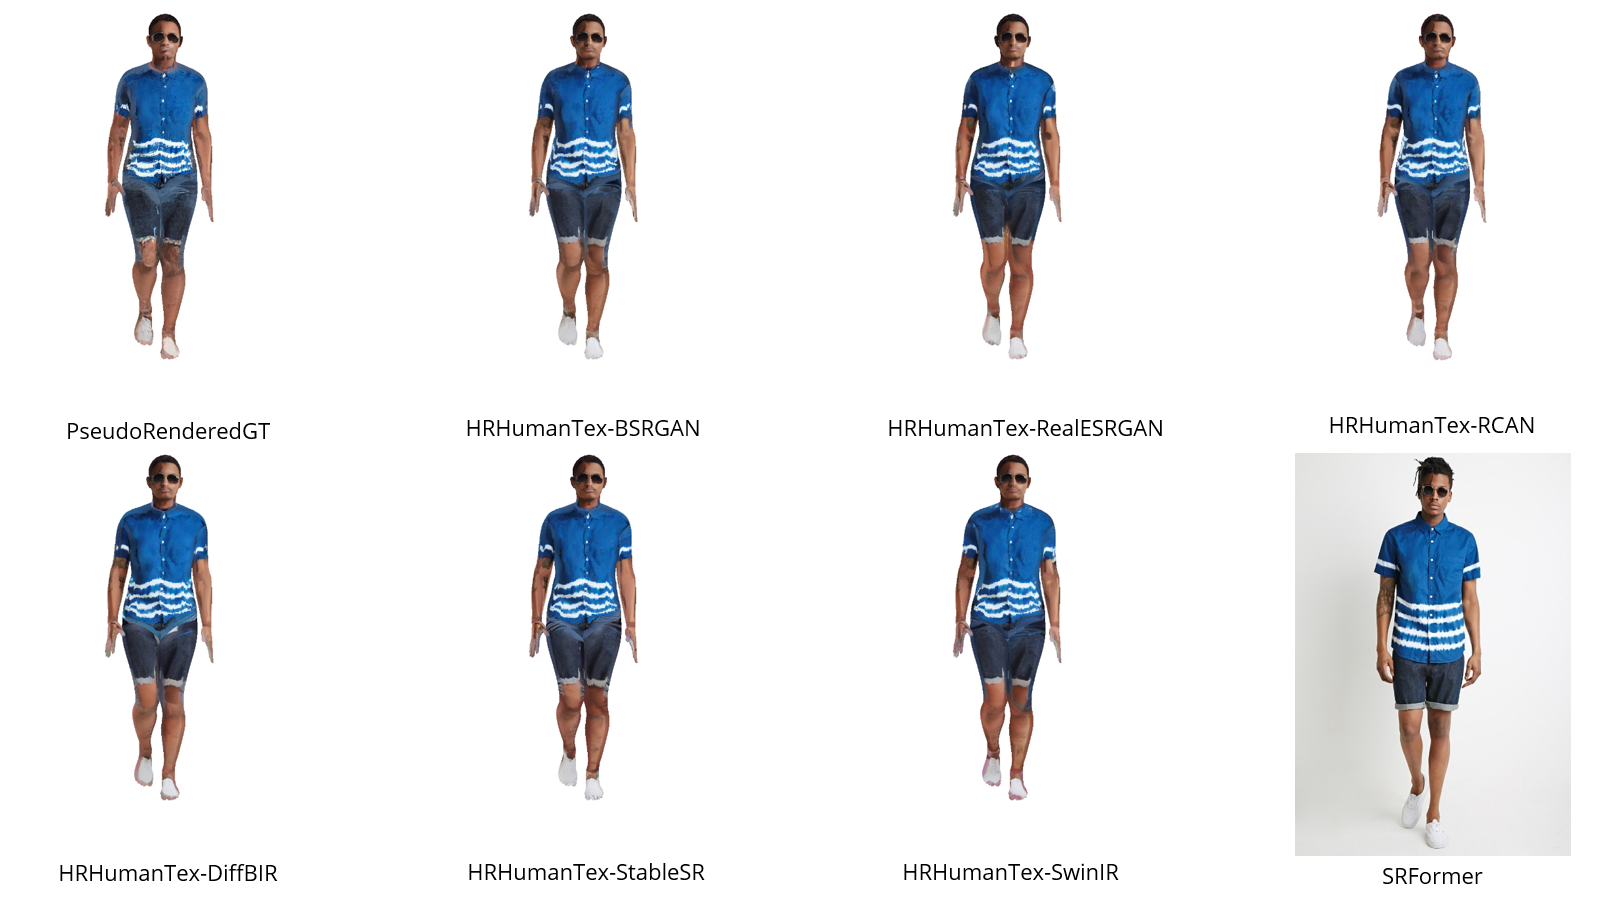
\includegraphics[width=1\textwidth]{fig/df10.png}
	\caption{ More qualitative visual comparison of different inpainting models in UV space and rendered images, data sampled from dataset DeepFashion~\cite{liuLQWTcvpr16DeepFashion}.}
	\label{fig:dfvis4}
\end{figure}

I first assess the quality of the inpainted UV textures directly in the texture space. Figure~\ref{fig:inpainteval3} and table~\ref{tab:inpaint_eval1} shows the PSNR, SSIM, LPIPS, and FID scores for textures produced by different inpainting models trained on super-resolved textures from various SR backbones, and Figure~\ref{fig:inpainteval2} and table~\ref{tab:render_inv_comparison}show evaluation results based on rendering. This evaluation dataset is samples from DeepFashion~\cite{liuLQWTcvpr16DeepFashion}. 

\subsection{Discussion}
By examining both the side-by-side texture visualizations and the quantitative scatter plots, one can clearly observe that nearly all HRHumanTex variants consistently outperform the original SMPLitex baseline. These models demonstrate the ability to generate high-resolution textures from a single input image with notable improvements in detail, fidelity, and spatial consistency.

This structured evaluation validated the effectiveness of the HRHumanTex framework, which not only adcances the original SMPLitex pipeline, but also delivers a pratical solution for downstream applications that demand high-quality 3D human textures.

According to the quantitative evaluation results, although SwinIR consistently achieves the best scores in UV-space metrics (SSIM and LPIPS), it tends to preserve structure without introducing hallucinated details. In contrast, DiffBIR often excels in rendering-based evaluations due to its capacity to enrich textures through diffusion-based generation, resulting in higher perceptual realism when textures are mapped onto a 3D body model.
This reflects a broader trend where models emphasizing fidelity (SwinIR, RCAN) perform better in UV metrics, while generative models (DiffBIR, RealESRGAN) produce visually richer, albeit less accurate, textures in render space.

These results suggest that high pixel similarity in UV space (PSNR/SSIM) does not always correlate with better rendered appearance. Perceptual metrics like LPIPS after projection are crucial for final quality assessment.

According to these evaluation results, inpainting model trained on SwinIR dataset and DiffBIR dataset perform very well and balanced in all indicators. So HRHumanTex-SwinIR and HRHumanTex-DiffBIR could both be the choice of high resolution texture estimation and inpainting.

